\documentclass{article}
\usepackage{amsmath}
\usepackage{amsthm}
\usepackage{amsfonts}
\usepackage{amssymb}
\usepackage{bbold}
\usepackage{dsfont}
\usepackage{graphicx}
\usepackage{cleveref}
\usepackage{bm}
\usepackage{booktabs}
\usepackage{siunitx}
\usepackage{xcolor}
\usepackage[utf8]{inputenc}
\usepackage[english]{babel}
\newtheorem{definition}{Definition}
\newtheorem{example}{Example}
\newcommand{\exP}[1]{\mathrm{e}^{#1}}
\newcommand{\dif}{\mathrm{d}}
\renewcommand{\vec}[1]{\mathbf{#1}}
\newcommand{\pdagger}{{\phantom{\dagger}}}
\newcommand{\state}[1]{\vert #1\rangle}
\newcommand{\cstate}[1]{\langle #1\vert}
\newcommand{\tr}[1]{\mathrm{tr}\left\{#1\right\}}
\newcommand{\trs}[2]{\, \mathrm{tr}_{#1}\{#2\}}
\newcommand{\expc}[3]{\langle #1\vert #2 \vert #3\rangle}
\usepackage[doi=false,url=false,isbn=false,backend=bibtex,style=nature,natbib=true,sorting=none]{biblatex}
\bibliography{bib.bib}
\usepackage{geometry}
\geometry{
	a4paper,
	total={170mm,257mm},
	left=20mm,
	top=20mm,
}
\begin{document}
\title{Report 11: Apparent bi-stability and Ehrenfest results of transport in the Fransson model}
\author{Rudolf Smorka}
\maketitle
\section{Uniqueness of steady state: Comparison between TTHEOM and MFHEOM}
System: $L=2$, spinfull with Peierls-type electron-phonon coupling. 
Parameters:
\begin{align*}
	t_0 &= \SI{40}{\milli\electronvolt}\\
	t_1 &= \SI{40}{\milli\electronvolt}\\
	\varepsilon_0 &= \SI{-240}{\milli\electronvolt}\\
	\omega_0 &= \SI{10}{\milli\electronvolt}\\
	\Gamma &= \SI{10}{\milli\electronvolt}\\
	T  &= \SI{25}{\milli\electronvolt}\\
	V & = \SI{0.48}{\volt}.
\end{align*}
\begin{figure}[!h]
	\centering
	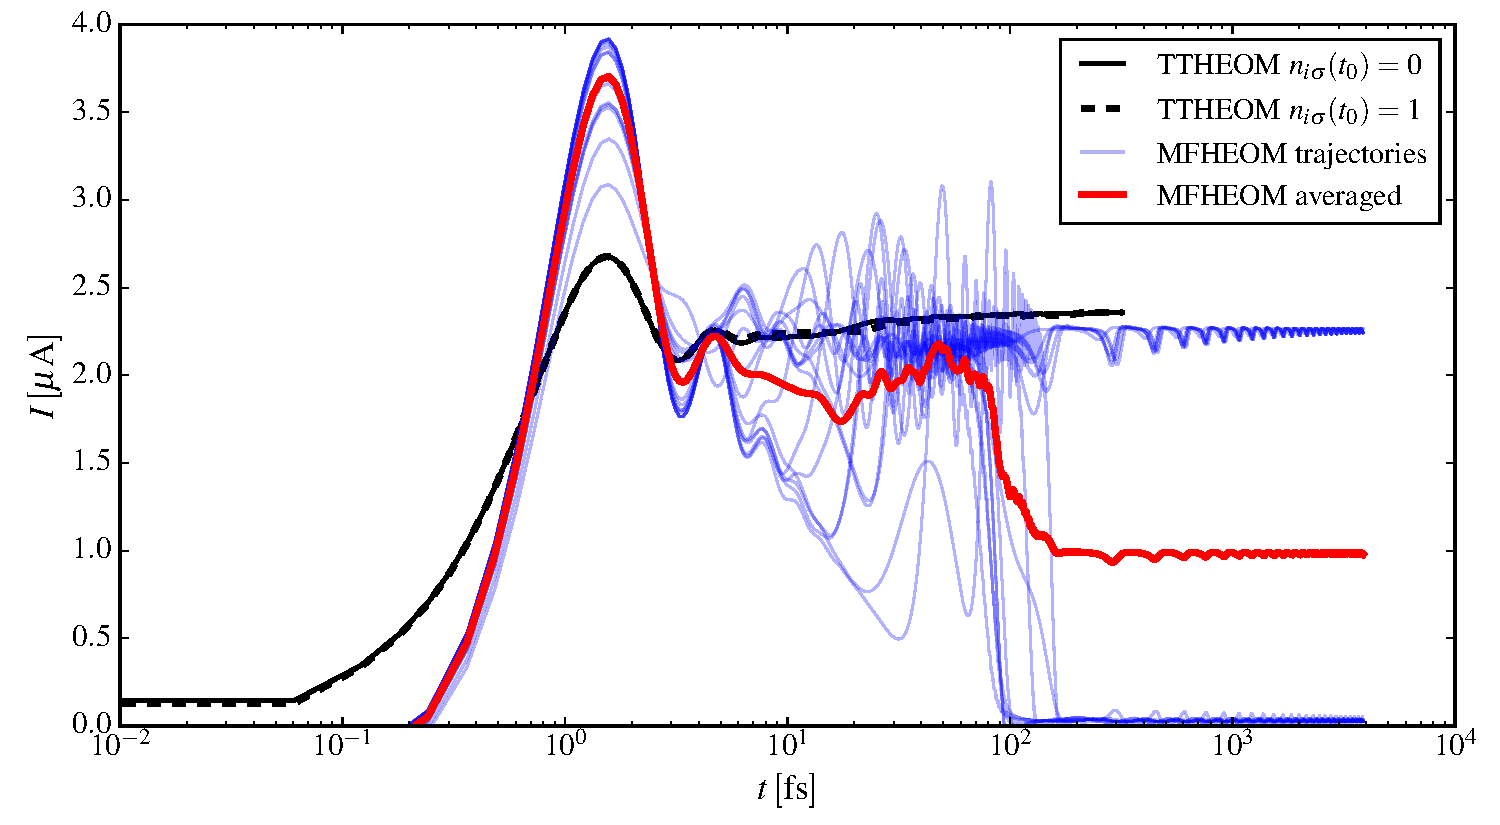
\includegraphics[width=1.0\textwidth]{figs/Fransson_L2_P0_non-unique_steady_state_currents_MFHEOM_vs_TTHEOM.pdf}
	\caption{Comparison of current dynamics: TTHEOM (black) with initially empty sites (full line), and initially occupied sites (dashed), and MFHEOM independent trajectories (blue lines) and average (red line).}
\end{figure}\\
Remarks:
\begin{itemize}
	\item TTHEOM norm of density operator is $0.992$ for the full and $0.991$ empty initial condition. The rank is set to $r=100$ and the vibrational mode is limited to have $n_v = $ 
	\item Within the Ehrenfest approach, the system has a bi-stability: If the initial momentum $P_0<P^*$, then the vibrational mode goes to a fix-point at $(X,P)=(-60,0)$. The corresponding steady-state current is finite. If $P_0>P^*$, then the fix-point is $(X,P) = (112,0)$ and the steady-state current vanishes. Based on the previous analysis of the model with Peierls-coupling (report 5), this result can be explained by the following: The single-particle eigenstates of the problem are $\varepsilon_{\pm\sigma} = \varepsilon_0 \pm \vert t_0+\sqrt{2\omega_0}t_1X\vert$. In order a charge current to flow, these levels have to be within the bias window $\mu_R<\varepsilon_{\pm\sigma}<\mu_L$. Plugging in the eigenenergies, one gets the inequality
	\begin{equation}
		X < \frac{\frac{V}{2}-t_0}{\sqrt{2\omega}t_1}\label{eq:X_ineq_Peierls}
	\end{equation} 
	as a necessary condition for a non-vanishing current. With the parameters above, the RHS of \cref{eq:X_ineq_Peierls} yields a value of $35.35$. Whenever the vibrational position exceeds this value, the levels are not within the bias window anymore, and charge current is zero. 
	Within the Ehrenfest-approach the potential of mean force is determined by the instantaneous electronic population, which, in turn, depends on the vibrational mode position and momentum. With this in mind, it easy to explain the bi-stability: If $P_0<P^*$, the first couple of time-steps, the position will decrease, which leads to a closing of the gap between electronic eigenenergies. Both levels can be populated due to coupling to the leads. When $P_0>P^*$, however, then the gap opens, leading to a finite population-difference $n_+-n_->0$ between eigenstates, and thus a finite force. The vibrational mode gets displaced even further such that the gap between eigenstates is so large, that both levels are outside the bias window. The lower level gets fully occupied, while the upper one remains unoccupied.
	\item This bi-stability is not observed in the full quantum problem, at least for the level of convergence set here. It is thus very likely an artifact of the Ehrenfest-approach.
\end{itemize}
\section{Fransson-model: Ehrenfest results}
\subsection{Averaged equilibrium density of states}
The density of states $\mathrm{DOS}_\alpha(\varepsilon)$ is computed for a single realization $\alpha$ of the vibrational position and momentum from the imaginary part of the retarded Green function $\bm{G}^R_\alpha(\varepsilon)$
\begin{align}
	\bm{G}^R_\alpha(\varepsilon)&= [\varepsilon\mathds{1}-\bm{H}_\alpha+\bm{\Sigma}^R]^{-1}\\
	\mathrm{DOS}_\alpha(\varepsilon) &= \frac{i}{\pi}\sum_{i} \mathrm{Im}([G^R_{ii}]_\alpha(\varepsilon)) 
\end{align}
with $\bm{\Sigma}^R = -\frac{i}{2}(\bm{\Gamma}_L+\bm{\Gamma}_R)$. For many realizations $N$ of vibrational positions and momenta, the averaged $\mathrm{DOS}(\varepsilon)$ is computed using a simple arithmetic average
\begin{equation}
	\mathrm{DOS}(\varepsilon) = \frac{1}{N}\sum_\alpha \mathrm{DOS}_\alpha(\varepsilon).
\end{equation}
The mode positions and momenta are sampled from the thermal Wigner distribution of a harmonic oscillator
\begin{equation}
	\rho(\{X\},\{P\}) =\prod_i  \frac{\alpha}{\pi}\exp\left[-\frac{2\alpha}{\omega}\left(\frac{P_i^2}{2}+\frac{\omega^2X_i^2}{2}\right)\right].
\end{equation}
The parameters are 
\begin{align*}
	\varepsilon_0 &= \SI{-240}{\milli\electronvolt}\\
	\omega_0 &= \SI{2}{\milli\electronvolt}\\
	t_0 &= \SI{40}{\milli\electronvolt}\\
	t_1 &= \SI{4}{\milli\electronvolt}\\
	\lambda_0 &= \SI{1}{\milli\electronvolt}\\
	\lambda_1 &= \SI{0.1}{\milli\electronvolt}\\
	\Gamma &= \SI{10}{\milli\electronvolt}\\
	T &= \SI{25}{\milli\electronvolt}
\end{align*}
which are the same as the ones used by Fransson, except that we use a slightly larger vibrational frequency (Fransson uses $\omega_0 = \SI{0.4}{\milli\electronvolt}$). 
\subsubsection{$L=2\times 4$}
\Cref{fig:DOS_2x4} shows the density of states for various lead spin-polarizations $P$ for a $L=2\times 4$ system. The feint orange line show the density of states for $t_1=\lambda_1 = \SI{0}{\electronvolt}$.  \Cref{fig:DOS_2x4_SP} (a) shows the difference in density of states for $P=0.5$ ($\mathrm{DOS}_\uparrow$) and $P=-0.5$ ($\mathrm{DOS}_\downarrow$) and (b) the integrated difference in density of states.
\color{red}{NEW DATA WITH FIXED HAMILTONIAN.}
\begin{figure}[!h]
	\centering
	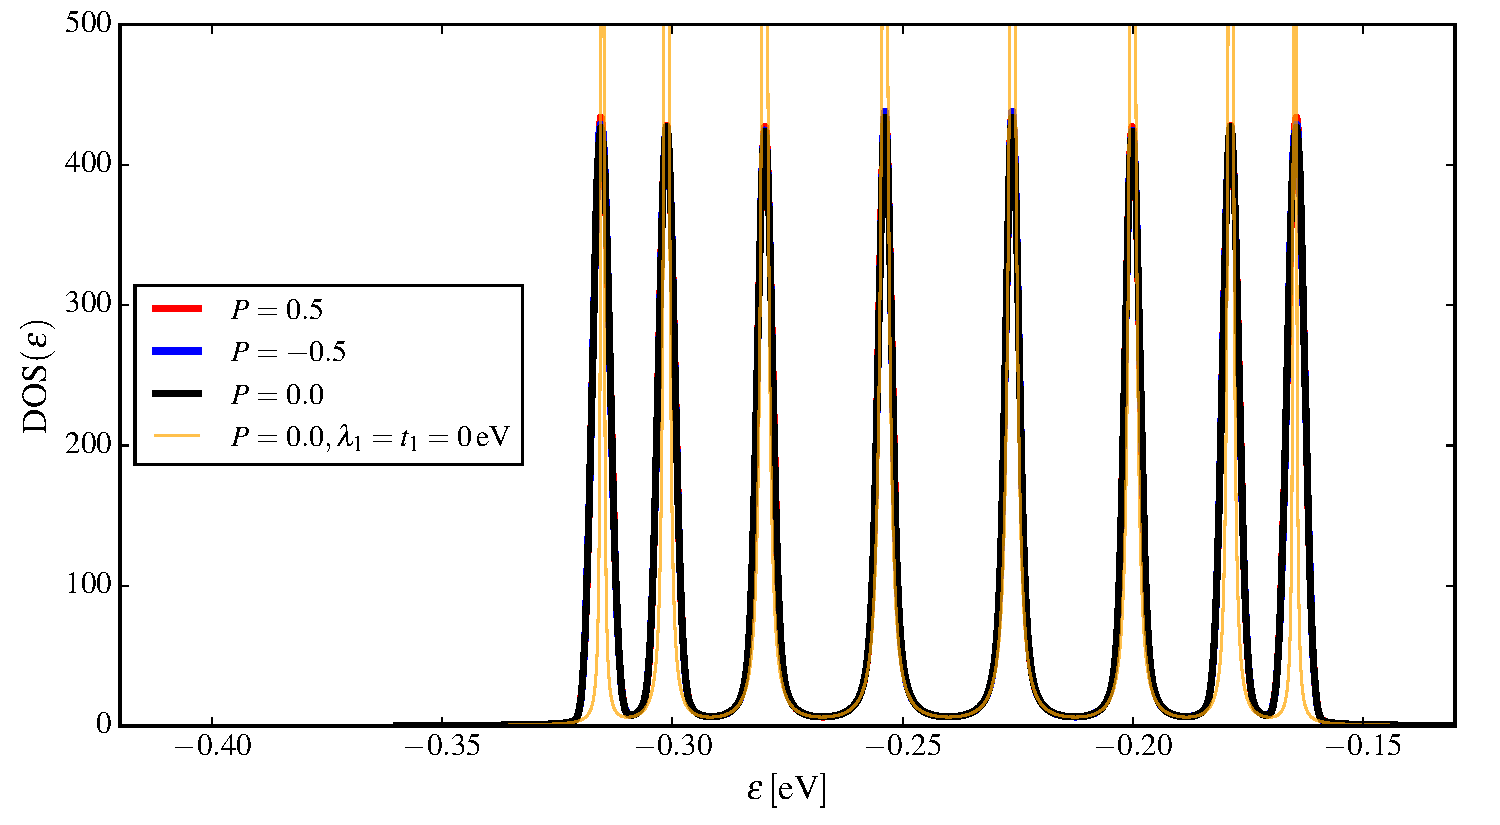
\includegraphics[width=0.9\textwidth]{figs/L2x4_Fransson_DOS_avg_1e5.pdf}
	\caption{Density of states for $P=0.5$ (red line), $P=-0.5$ (blue line), $P=0.0$ (black line) and for $\lambda_1=t_1=\SI{0}{\electronvolt}$ (orange line).}\label{fig:DOS_2x4}
\end{figure}
\begin{figure}[!h]
	\centering
	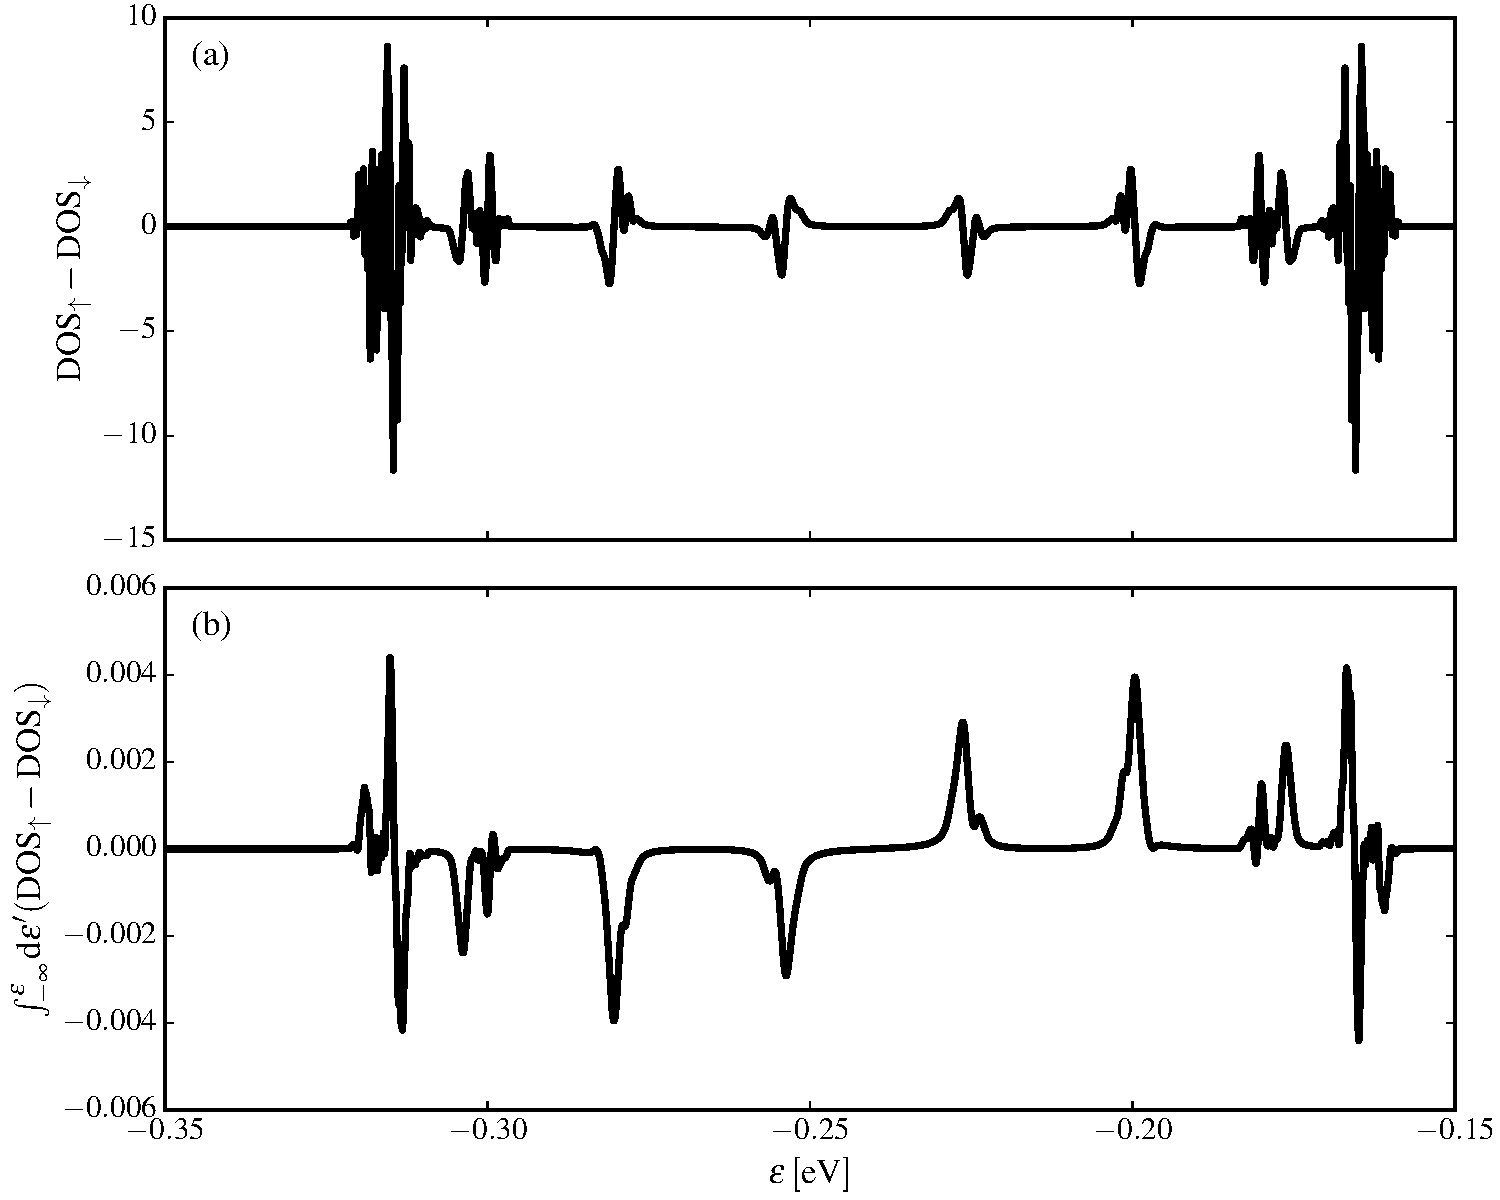
\includegraphics[width=0.9\textwidth]{figs/L2x4_Fransson_diff_DOS_avg_1e5.pdf}
	\caption{Lead-induced spin polarization in density of states (a) and integrated polarization (b).}\label{fig:DOS_2x4_SP}
\end{figure}
\clearpage
\subsubsection{$L=4\times 4$}
\begin{figure}[!h]
	\centering
	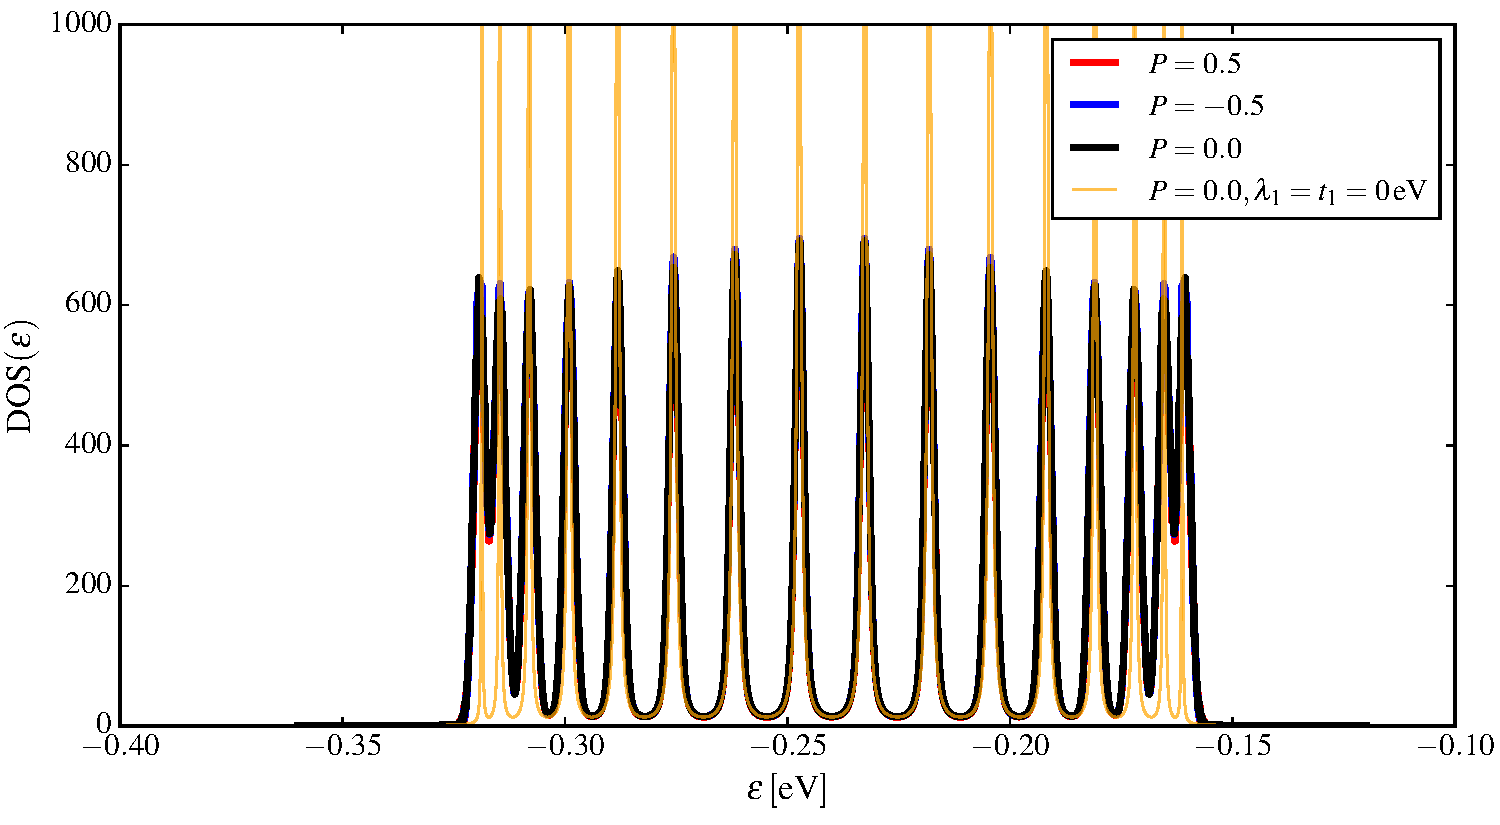
\includegraphics[width=0.9\textwidth]{figs/L4x4_Fransson_DOS_avg_27000.pdf}
	\caption{Density of states for $P=0.5$ (red line), $P=-0.5$ (blue line), $P=0.0$ (black line) and for $\lambda_1=t_1=\SI{0}{\electronvolt}$ (orange line).}
\end{figure}
\begin{figure}[!h]
	\centering
	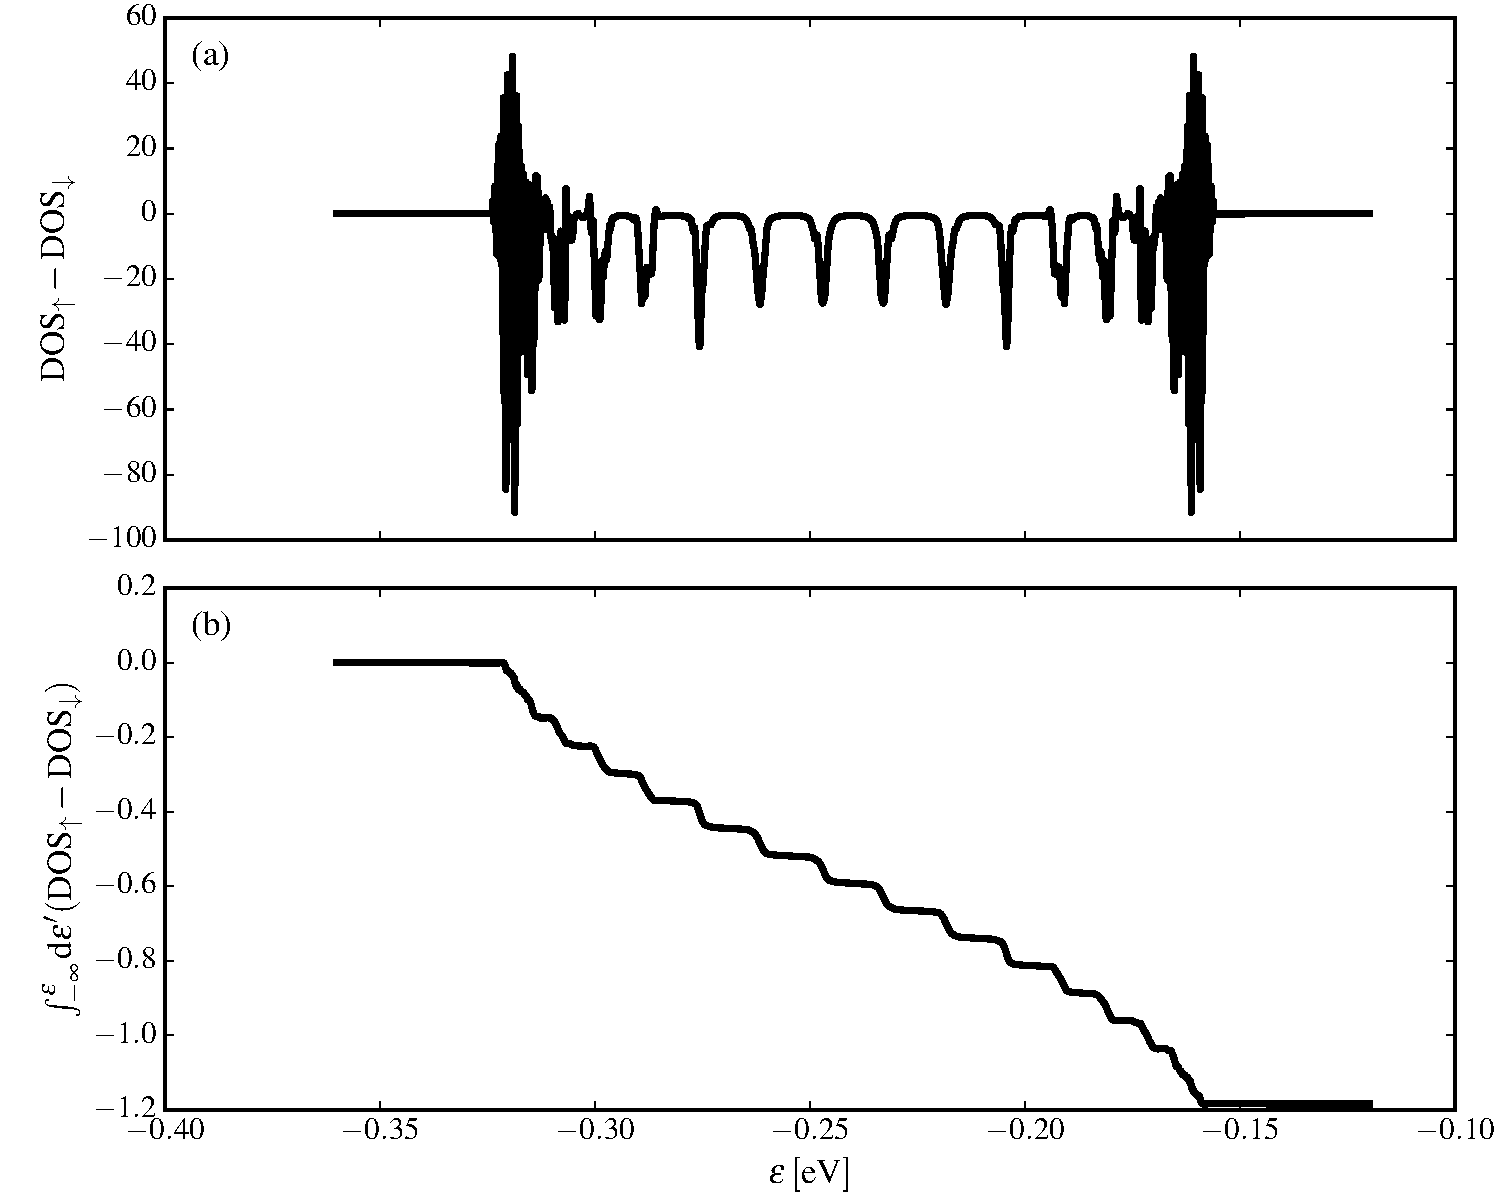
\includegraphics[width=0.9\textwidth]{figs/L4x4_Fransson_diff_DOS_avg_27000.pdf}
	\caption{Lead-induced spin polarization in density of states (a) and integrated polarization (b).}
\end{figure}
\subsubsection{Remarks}
\begin{itemize}
	\item The vibrational coupling broadens mostly states at the band edges. 
	States in the center are practically unaffected by the vibrations. 
	This in contrast to Fig. 1 in \cite{fransson2020vibrational}, which shows that the vibrational coupling leads to an exchange-splitting of states independent of energy.
	\item The difference in density of states 
	\item The integrated difference in density of states is anti-symmetric around Fermi-level. Within the assumption, that the vibrational distribution is in equilibrium, a vanishing magnetoresistance for very high bias is expected. For intermediate bias, there might be a finite magnetoresistance. 
	\item The averaged density of states does not reflect the full Ehrenfest calculation, as vibrational relaxation and other effects, arising due to feedback between electronic subsystem and vibrational subsystem, are neglected. The result is a time-dependent density of states, which will be shown below.
\end{itemize}
\subsection{Time-dependent density of states under trajectory-averaged vibrational positions and momenta}
Given trajectory-averaged vibrational positions $\{\bar{X}(t)\}$ and momenta $\{\bar{P}(t)\}$, the density of states of the coupled molecule is computed using Greens functions as above, but now for each time.
\subsection{Averaged density of states in the steady-state}

\subsection{Electronic dynamics}

\subsection{Vibrational dynamics}
\subsubsection{Remarks}
\begin{itemize}
	\item All vibrational modes ''relax'' to the same steady-state position and momentum. 
	\item For each trajectory independently, only the first mode relaxes. For all other modes, each trajectory reaches a limit cycle, where the bond mode oscillates around the mean-field minimum. Upon increasing the number of trajectories, the typical limit-cycle amplitude of the vibrational position decreases. It is very likely, that the limit-cycle is a finite-trajectory artifact.
\end{itemize}
\subsection{Current and magnetoresistance dynamics}
\printbibliography
\end{document}




